\documentclass[11pt]{article}
\usepackage[utf8]{inputenc}	% Para caracteres en español
\usepackage{amsmath,amsthm,amsfonts,amssymb,amscd}
\usepackage{multirow,booktabs}
\usepackage[table]{xcolor}
\usepackage{fullpage}
\usepackage{lastpage}
\usepackage{enumitem}
\usepackage{fancyhdr}
\usepackage{mathrsfs}
\usepackage{wrapfig}
\usepackage{setspace}
\usepackage{calc}
\usepackage{multicol}
\usepackage{cancel}
\usepackage{float}
\usepackage{physics}
\usepackage[retainorgcmds]{IEEEtrantools}
\usepackage[margin=1cm]{geometry}
\usepackage{amsmath}
\newlength{\tabcont}
\setlength{\headheight}{14pt}
\setlength{\parindent}{0.0in}
\setlength{\parskip}{0.05in}
\usepackage{empheq}
\usepackage{framed}
\usepackage[most]{tcolorbox}
\usepackage{xcolor}
\usepackage[version=3]{mhchem}
\usepackage[english]{babel}
\usepackage[utf8]{inputenc}
\usepackage{graphicx}
\usepackage[colorinlistoftodos]{todonotes}
\usepackage{mdframed}

\colorlet{shadecolor}{orange!15}
\parindent 0in
\parskip 12pt
\geometry{margin=1in, headsep=0.45in}
\theoremstyle{definition}
\newtheorem{defn}{Definition}
\newtheorem{reg}{Rule}
\newtheorem{exer}{Exercise}
\newtheorem{note}{Note}
\begin{document}
\setcounter{section}{2}
%\setcounter{subsection}{}
\title{Problem Set 9}

%==============================================================
%\thispagestyle{empty}
\pagestyle{fancy}
\fancyhf{}
\rhead{Physics 180}
\chead{Problem Set 9}
\lhead{Olyn D. Desabelle}
\rfoot{Page \thepage}

\begin{center}
{\LARGE \bf Problem Set 9}\\
%{\large Physics 180}\\
%Olyn D. Desabelle
\end{center}

\begin{figure}[H]
    \centering
    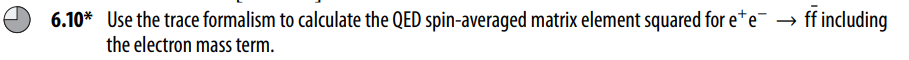
\includegraphics[scale = 0.5]{6.10.png}
\end{figure}

$e^+e^- \to f\bar{f}$ gives the following LO Feynmann diagram as given in Thomson:

\begin{figure}[H]
    \centering
    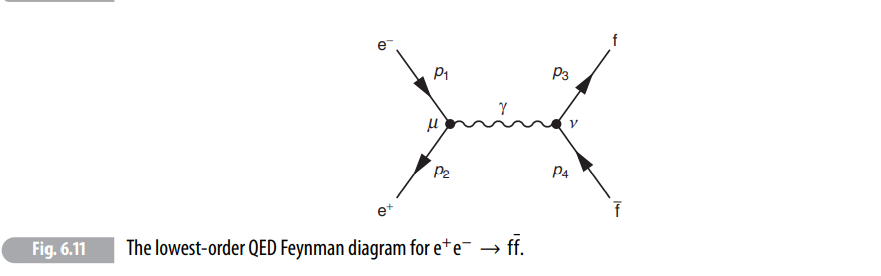
\includegraphics[scale = 0.5]{fig 6.11.png}
\end{figure}

With this, we may use QED rules to get the matrix elements, noting the additional charge of the fermion $Q_f$:

\begin{align}
    -i\mathcal{M}_{fi} &= Q_f[\bar{v}(p_2)ie\gamma^{\mu}u(p_1)] 
    \left[ \frac{-ig_{\mu\nu}}{q^2} \right]
    [\bar{u}(p_3)ie\gamma^{\nu}u(p_4)]\\
    \mathcal{M}_{fi} &= -Q_f[\bar{v}(p_2)e\gamma^{\mu}u(p_1)] 
    \left[ \frac{g_{\mu\nu}}{q^2} \right]
    [\bar{u}(p_3)e\gamma^{\nu}u(p_4)]\\
    \mathcal{M}_{fi} &= \frac{-Q_fe^2}{q^2} [\bar{v}(p_2)\gamma^{\mu}u(p_1)]
    g_{\mu\nu}[\bar{u}(p_3)\gamma^{\nu}u(p_4)]\\
    \mathcal{M}_{fi} &= \frac{-Q_fe^2}{q^2} [\bar{v}(p_2)\gamma^{\mu}u(p_1)]
    [\bar{u}(p_3)\gamma_{\nu}u(p_4)]\\
\end{align}

we may rearrange the elements in trace formalism as in Equation (6.51) to get the spin-summed matrix element squared $\sum_{\text{spins}} |\mathcal{M}_{fi}|^2$:

\begin{align}
    \sum_{\text{spins}} |\mathcal{M}_{fi}|^2  &= \frac{Q_f^2e^4}{q^4} 
    \Trace([\cancel{p}_2-m_e]\gamma^{\mu}[\cancel{p}_1+m_e]\gamma^{\nu}) \times 
    \Trace([\cancel{p}_3+m_f]\gamma_{\mu}[\cancel{p}_4-m_f]\gamma_{\nu})
\end{align}

we proceed with evaluating the traces:

\begin{align}
    \Trace([\cancel{p}_2-m_e]\gamma^{\mu}[\cancel{p}_1+m_e]\gamma^{\nu}) &=
    \Trace(\cancel{p}_2\gamma^{\mu}\cancel{p}_1\gamma^{\nu} 
    + \cancel{p}_2\gamma^{\mu}m_e\gamma^{\nu}
    - \cancel{p}_1\gamma^{\nu}m_e\gamma^{\mu}
    - m_e^2\gamma^{\mu}\gamma^{\nu}
    )\\
\end{align}

we may rewrite $\cancel{p}_1 = \gamma^{\sigma}p_{1\sigma}$ and $\cancel{p}_2 = \gamma^{\rho}p_{2\rho}$, thus we have:

\begin{align}
    \Trace([\gamma^{\rho}p_{2\rho}-m_e]\gamma^{\mu}[\gamma^{\sigma}p_{1\sigma}+m_e]\gamma^{\nu}) &=
    \Trace(\gamma^{\rho}p_{2\rho}\gamma^{\mu}\gamma^{\sigma}p_{1\sigma}\gamma^{\nu} 
    + \gamma^{\rho}p_{2\rho}\gamma^{\mu}m_e\gamma^{\nu}
    \\ &- \gamma^{\sigma}p_{1\sigma}\gamma^{\nu}m_e\gamma^{\mu}
    - m_e^2\gamma^{\mu}\gamma^{\nu}
    )
\end{align}

we note the following trace theorems:

\begin{align*}
    &\text{(b) the trace of odd-numbered $\gamma$-matrices zero out}\\
    &\text{(c) }\Trace(\gamma^{\mu}\gamma^{\nu}) = 4g^{\mu\nu}\\
    &\text{(d) }\Trace(\gamma^{\mu}\gamma^{\nu}\gamma^{\rho}\gamma^{\sigma}) = 4g^{\mu\nu}g^{\rho\sigma} - 4g^{\mu\rho}g^{\nu\sigma} + 4g^{\mu\sigma}g^{\nu\rho}
\end{align*}

with these, our trace becomes:

\begin{align}
    \Trace([\cancel{p}_2-m_e]\gamma^{\mu}[\cancel{p}_1+m_e]\gamma^{\nu}) 
    &=
    \Trace(
        \gamma^{\rho}p_{2\rho}\gamma^{\mu}\gamma^{\sigma}p_{1\sigma}\gamma^{\nu} 
    ) - m_e^2\Trace(\gamma^{\mu}\gamma^{\nu})\\
    &=
    p_{2\rho}p_{1\sigma}\Trace(
        \gamma^{\rho}\gamma^{\mu}\gamma^{\sigma}\gamma^{\nu} 
    ) - m_e^2\Trace(\gamma^{\mu}\gamma^{\nu})\\
    &= 
    4p_{2\rho}p_{1\sigma}(
       g^{\rho\mu}g^{\sigma\nu} - g^{\rho\sigma}g^{\mu\nu} + g^{\rho\nu}g^{\mu\sigma}
    )
    - 4m_e^2g^{\mu\nu}\\
    &= 
    4p_2^{\mu}p_1^{\nu} - 4g^{\mu\nu}(p_1\cdot p_2) + 4p_2^{\nu}p_1^{\mu}
    - 4m_e^2g^{\mu\nu}\\
\end{align}

we do the same steps for the other trace:

\begin{align}
    \Trace([\cancel{p}_3+m_f]\gamma_{\mu}[\cancel{p}_4-m_f]\gamma_{\nu}) &=
    \Trace(\cancel{p}_3\gamma_{\mu}\cancel{p}_4\gamma_{\nu}
    - \cancel{p}_3\gamma_{\mu} m_f \gamma_{\nu}
    + m_f\gamma_{\mu} \cancel{p}_4 \gamma_{\nu} 
    - m_f^2\gamma_{\mu}\gamma_{\nu}
    )\\
    &=
    \Trace(
    \gamma^{\rho}p_{3\rho}\gamma_{\mu}\gamma^{\sigma}p_{4\sigma}\gamma_{\nu}
    - \gamma^{\rho}p_{3\rho}\gamma_{\mu} m_f \gamma_{\nu}\\
    &\;\;\;\;\;\;\;\;\; + m_f\gamma_{\mu} \gamma^{\sigma}p_{4\sigma} \gamma_{\nu} 
    - m_f^2\gamma_{\mu}\gamma_{\nu}
    )\\
    &=
    p_{3\rho}p_{4\sigma}\Trace(\gamma^{\rho}\gamma_{\mu}\gamma^{\sigma}\gamma_{\nu} ) - m_f^2\Trace(\gamma_{\mu}\gamma_{\nu})\\
    &=
    4p_{3\mu}p_{4\nu} - 4g_{\mu\nu}(p_3 \cdot p_4) + 4p_{3\nu}p_{4\mu} - 4m_f^2g_{\mu\nu}
\end{align}

thus the spin-summed matrix element squared becomes:

\begin{align}
    \sum_{\text{spins}} |\mathcal{M}_{fi}|^2  &= \frac{Q_f^2e^4}{q^4} 
    \left( 4p_2^{\mu}p_1^{\nu} - 4g^{\mu\nu}(p_1\cdot p_2) + 4p_2^{\nu}p_1^{\mu}
    - 4m_e^2g^{\mu\nu} \right)
    \times\\
    &\;\;\;\;\;\;\;\;\;\;\;\;\;\;\; \left( 4p_{3\mu}p_{4\nu} - 4g_{\mu\nu}(p_3 \cdot p_4) + 4p_{3\nu}p_{4\mu} - 4m_f^2g_{\mu\nu} \right)\\
    &= \frac{16Q_f^2e^4}{q^4} 
    \left( p_2^{\mu}p_1^{\nu} - g^{\mu\nu}(p_1\cdot p_2) + p_2^{\nu}p_1^{\mu}
    - m_e^2g^{\mu\nu} \right)
    \times\\
    &\;\;\;\;\;\;\;\;\;\;\;\;\;\;\; \left( p_{3\mu}p_{4\nu} - g_{\mu\nu}(p_3 \cdot p_4) + p_{3\nu}p_{4\mu} - m_f^2g_{\mu\nu} \right)\\
\end{align}

we may contract the indices using the following:

\begin{align*}
    g^{\mu\nu}g_{\mu\nu} = 4
    \;\;\;
    p_2^{\mu}p_1^{\nu}g_{\mu\nu} = (p_1 \cdot p_2)
    \;\;\;
    p_2^{\mu}p_1^{\nu}p_{3\mu}p_{4\nu} = (p_2 \cdot p_3)(p_1 \cdot p_4)
\end{align*}

thus we have:

\begin{align}
    \sum_{\text{spins}} |\mathcal{M}_{fi}|^2  = \frac{16Q_f^2e^4}{q^4}
    &\biggl(
    (p_1 \cdot p_4) (p_2 \cdot p_3)
    - (p_1 \cdot p_2) (p_3 \cdot p_4)
    + (p_1 \cdot p_3)(p_2 \cdot p_4)
    -m_f^2(p_1 \cdot p_2)\\  
     &- (p_1 \cdot p_2)(p_3 \cdot p_4)
     + 4(p_1 \cdot p_2)(p_3 \cdot p_4)
     - (p_1 \cdot p_2)(p_3 \cdot p_4)
     + 4m_f^2(p_1 \cdot p_2)\\
    &+ (p_1 \cdot p_3) (p_2 \cdot p_4)
    -(p_1 \cdot p_2) (p_3 \cdot p_4)
    +(p_1 \cdot p_4) (p_2 \cdot p_3)
    - m_f^2 (p_1 \cdot p_2)\\
        &- m_e^2(p_3 \cdot p_4) 
        + 4m_e^2(p_3 \cdot p_4)
        - m_e^2(p_3 \cdot p_4)
        + 4m_e^2m_f^2
    \biggr)
\end{align}

\begin{align}
    \sum_{\text{spins}} |\mathcal{M}_{fi}|^2  &= \frac{16Q_f^2e^4}{q^4}
    \left(
        2(p_1 \cdot p_4) (p_2 \cdot p_3)
        + 2(p_1 \cdot p_3) (p_2 \cdot p_4)
        + 2m_f^2(p_1 \cdot p_2)
        + 2m_e^2(p_3 \cdot p_4)
        + 4m_e^2m_f^2  
    \right)\\
    &= \frac{32Q_f^2e^4}{q^4}
    \left(
        (p_1 \cdot p_4) (p_2 \cdot p_3)
        + (p_1 \cdot p_3) (p_2 \cdot p_4)
        + m_f^2(p_1 \cdot p_2)
        + m_e^2(p_3 \cdot p_4)
        + 2m_e^2m_f^2  
    \right)\\
\end{align}

to get the spin-averaged matrix element squared, we evaluate:

\begin{align}
    \expval{|\mathcal{M}_{fi}|^2} &= \frac{1}{4}\sum_{\text{spins}} |\mathcal{M}_{fi}|^2\\  
\end{align}

from the spin-summed matrix element squared, then we have:

\begin{align}
    \expval{|\mathcal{M}_{fi}|^2}
    =
    \frac{8Q_f^2e^4}{q^4}
    \left[
        (p_1 \cdot p_4) (p_2 \cdot p_3)
        + (p_1 \cdot p_3) (p_2 \cdot p_4)
        + m_f^2(p_1 \cdot p_2)
        + m_e^2(p_3 \cdot p_4)
        + 2m_e^2m_f^2  
    \right]
\end{align}

we may rewrite the four-momentum squared of the virtual phton as $q^2=(p_1+p_2)^2$, thus getting:

\begin{equation}
\boxed{
    \expval{|\mathcal{M}_{fi}|^2}
    =
    \frac{8Q_f^2e^4}{(p_1+p_2)^4}
    \left[
        (p_1 \cdot p_4) (p_2 \cdot p_3)
        + (p_1 \cdot p_3) (p_2 \cdot p_4)
        + m_f^2(p_1 \cdot p_2)
        + m_e^2(p_3 \cdot p_4)
        + 2m_e^2m_f^2  
    \right]
}
\end{equation}

%from this we may get the spin-averaged matrix element squared $\expval{|\mathcal{M}_{fi}|^2}$:



%==============================================================
\end{document}